\section{Pianificazione dei test}

Si vuole adottare una strategia di verifica del software tramite test opportunamente predeterminati e che garantiscano almeno un test per ogni requisito. I test sono l'applicazione delle tecniche di verifica dinamica introdotte nelle \NormeDiProgetto{}; tali attività, oltre a richiedere l'esecuzione del programma, devono poter essere ripetibili, ossia tramite delle specifiche su come riprodurre i test vogliamo che il loro output sia deterministico. \`E importante che i test di unità vengano svolti in parallelo, dando precedenza alle unità che producono risultati utili alla comprensione del loro funzionamento integrato, l'ambiente di testing deve soddisfare tale obiettivo. \\
L'attività di test deve produrre un \glossario{log} che specifica quando e chi ha eseguito il test e con quali input; l'insorgenza di \glossario{failure} deve essere tracciata e catalogata.

	\subsection{Livelli di testing}
	Il testing del software viene suddiviso in livelli differenti e si concretizzano in un esecuzione bottom-up che avanza sequenzialmente alle attività di codifica e  di validazione. 
	I test che si andranno ad applicare sono di cinque tipi, riservando la specifica delle ultime due tipologie alla prossima revisione:

\begin{enumerate}
	\item Test di Validazione (TV): viene verificato che il prodotto soddisfi quanto richiesto dal \glossario{proponente} individuando delle macro azioni da eseguire sul sistema che un normale utente svolge comunemente;
	\item Test di Sistema (TS): sono test relativi al comportamento dell'intero sistema ossia viene verificato che la sua architettura generale funziona complessivamente bene;
	\item Test di Integrazione (TI): vengono verificate le componenti del sistema contenute nella \SpecificaTecnica{}, ossia viene verificato che i \glossario{package} siano funzionanti e in grado di funzionare nel loro insieme; %PACKAGE
	\item Test di Unità (TU): viene testata ogni unità, ossia la più piccola parte di lavoro assegnabile ad un programmatore. In questo progetto una unità dovrebbe corrispondere ad una \code{function} o a un \code{method};  %FUNCION METODI
	\item Test di Regressione (TR): possono essere test di tutte le tipologie succitate che devono mostrare il funzionamento del prodotto a seguito di una modifica.
\end{enumerate}

	La figura \ref{fig:V-Model} illustra come i test elencati vengono distribuiti durante in ciclo di vita del prodotto.

	\begin{figure}[H]
	\centering 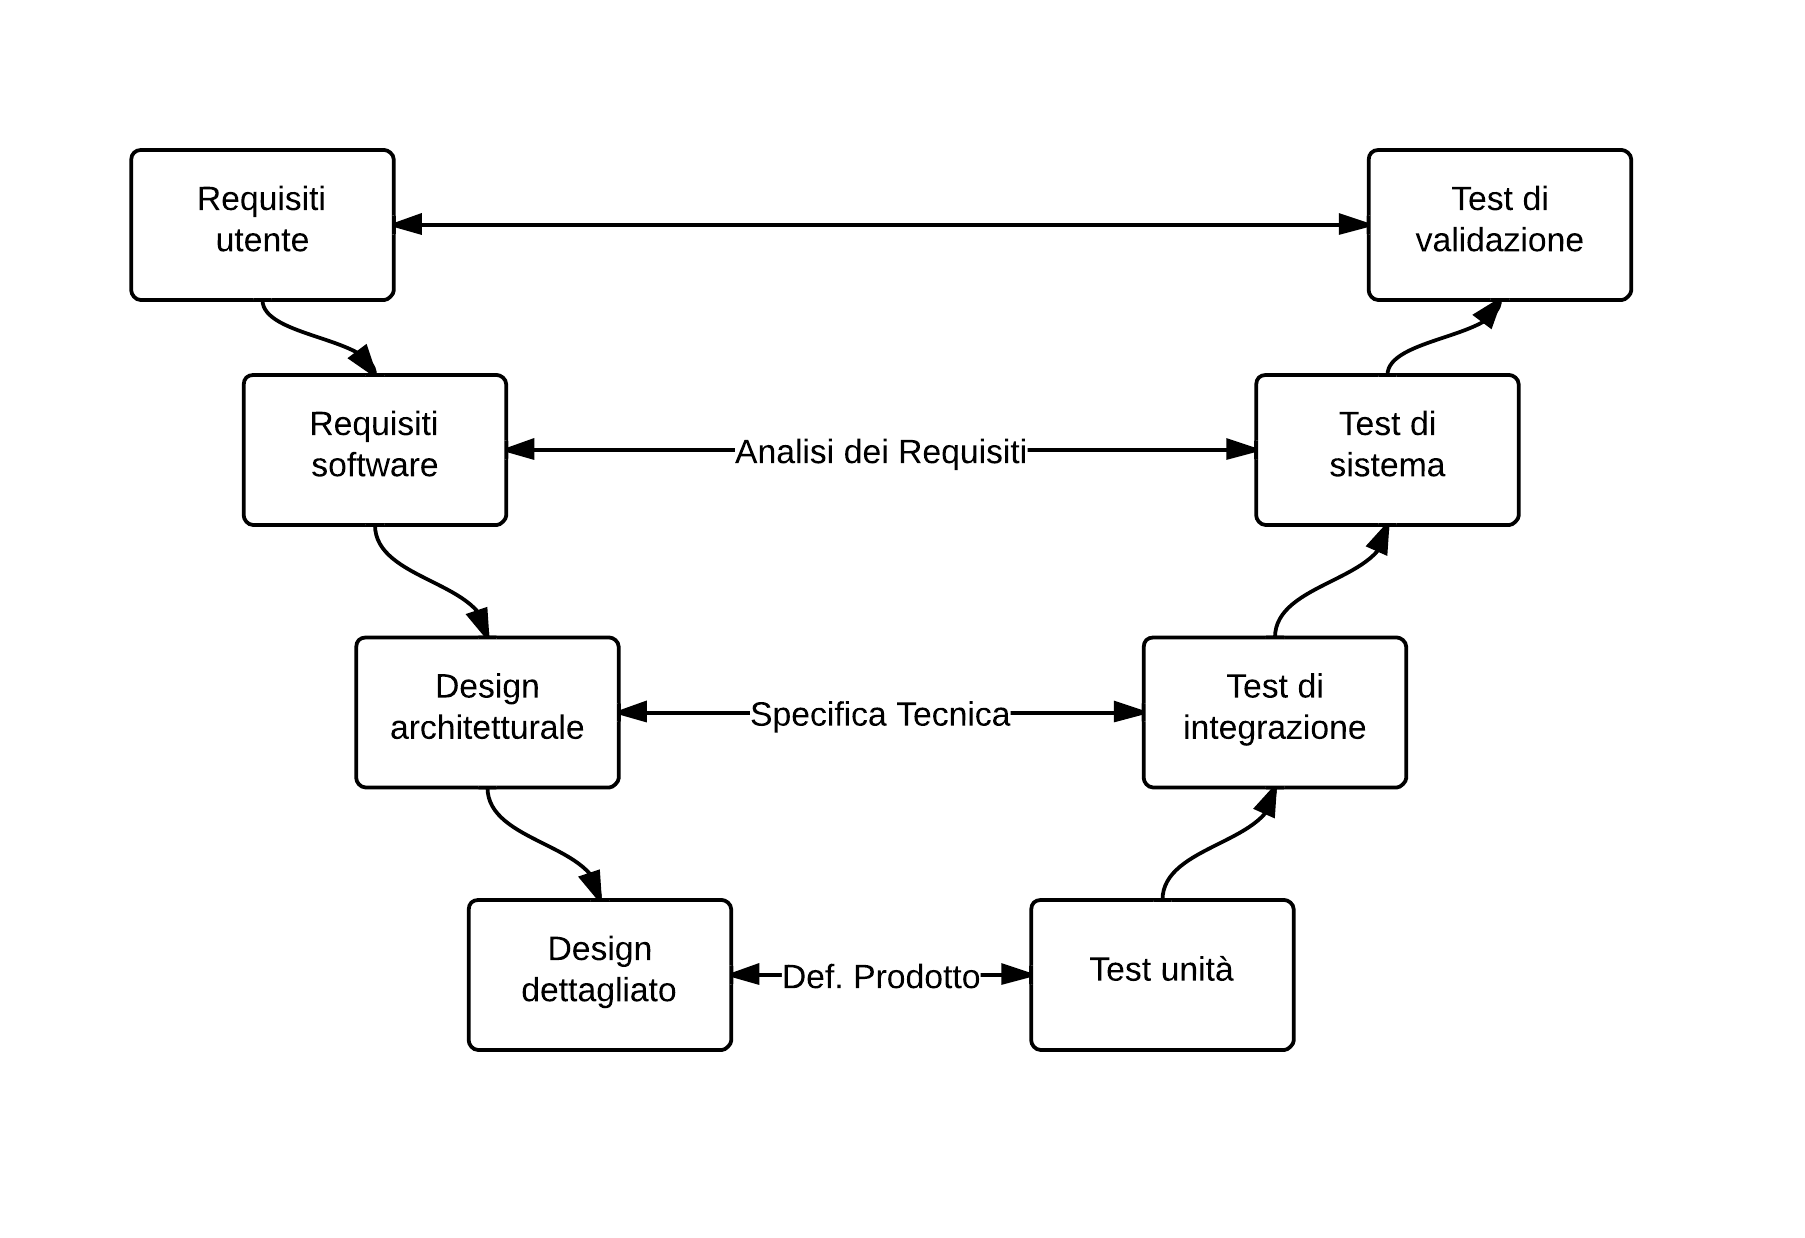
\includegraphics[width=1\textwidth]{V-Model.png}
	\caption{V-Model per il testing software}
	\label{fig:V-Model}
	\end{figure}

	\subsection{Test di sistema}
	Vengono qui descritti i test di sistema che andranno a verificare il funzionamento complessivo delle componenti.
	
	%TODO qui va la tabella descrzione dei TS / requisiti
	
	\subsection{Test di integrazione}
	I test di integrazione vanno a controllare il corretto funzionamento delle componenti descritti dalla progettazione ad alto livello. Si è scelto di utilizzare un approccio \glossario{top-down} ad eccezione del test TI 10 che viene eseguito con la metodologia \glossario{bottom-up}. Di seguito viene riportato un diagramma informale per chiarire l'albero dei test di integrazione.

	\begin{figure}[H]
	\centering 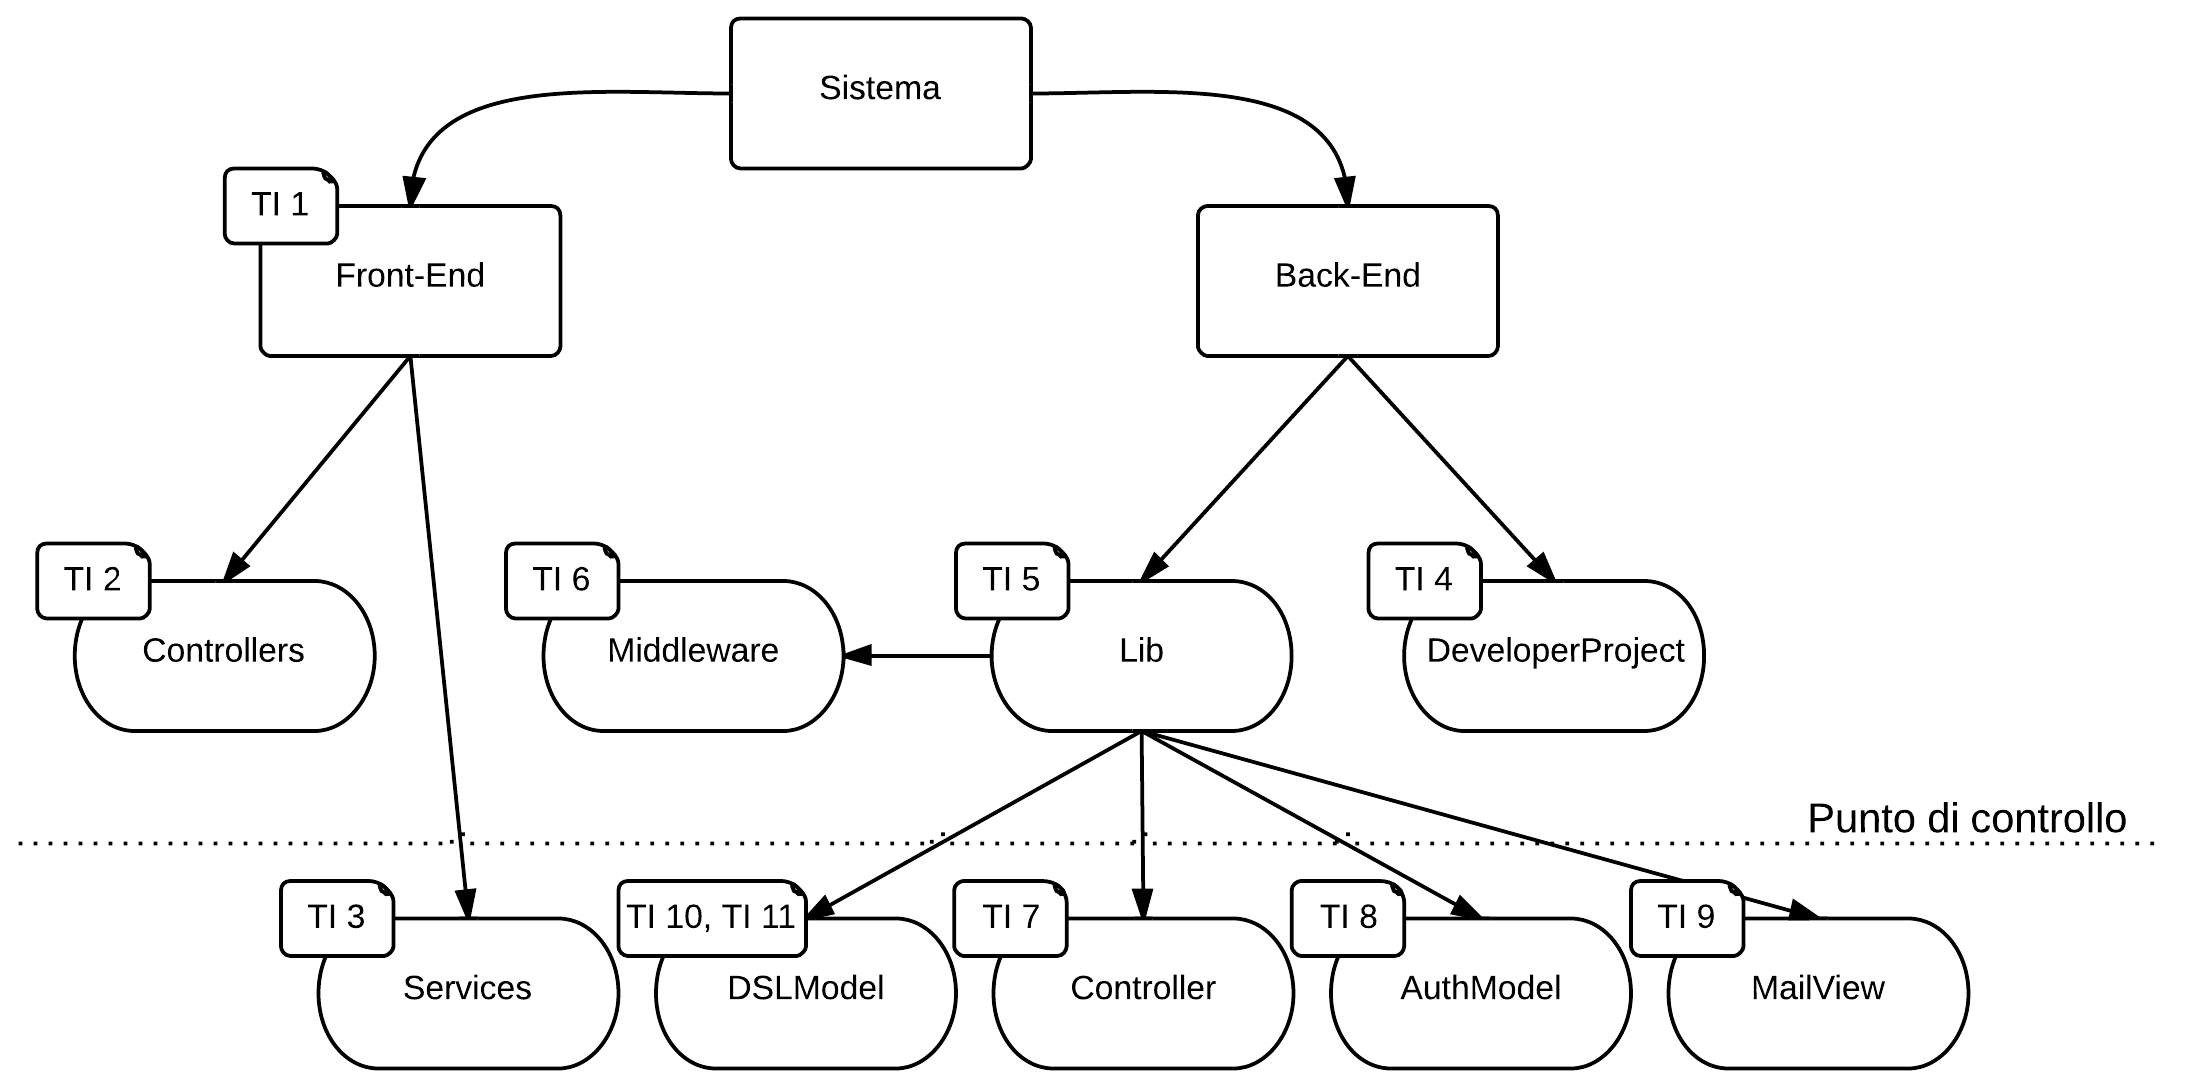
\includegraphics[width=1\textwidth]{sequenza-di-integrazione.png}
	\caption{Sequenza d'integrazione delle componenti}
	\label{fig:sequenza-di-integrazione}
	\end{figure}

	Con la tecnica \glossario{top-down} le componenti di più alto livello sono testate non appena sono implementate. Le componenti del sottosistema che non sono ancora state sviluppate, vengono simulate dagli \glossario{stub}. Man mano che si procede con la codifica delle componenti di più basso livello, queste vengono integrate e viene eseguito il relativo test. Grazie all'integrazione incrementale delle componenti del sistema, è più semplice determinare quale componente crea problemi e le funzioni di più alto livello sono testate prima.

	\begin{figure}[H]
	\centering 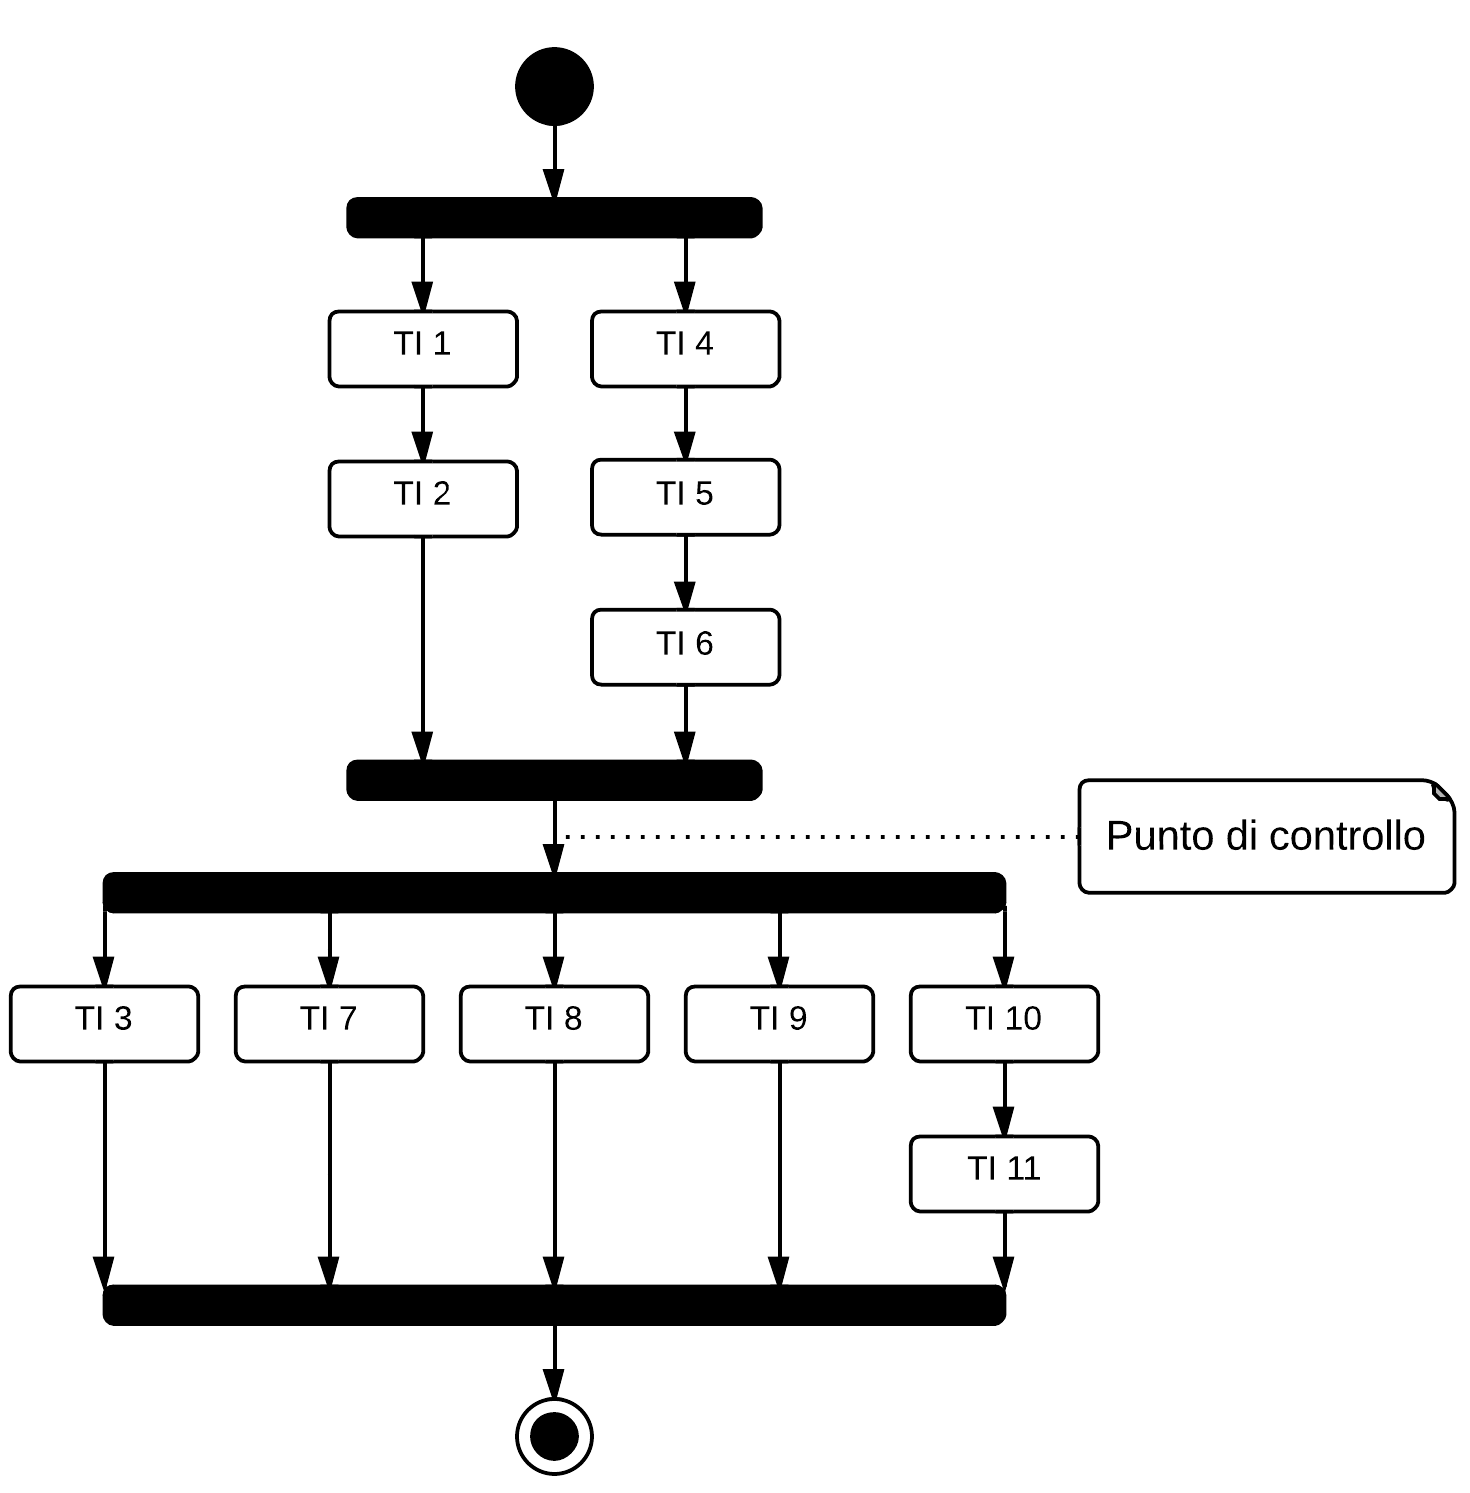
\includegraphics[width=0.57\textwidth]{sequenza-dei-test.png}
	\caption{Diagramma di attività dei test}
	\label{fig:sequenza-dei-test}
	\end{figure}
	
	%TODO tabella: componente / test
	\bgroup
	\begin{longtable}[H]{|P{1cm}|P{5cm}|P{4.5cm}|P{2cm}|}
		\hline \textbf{Test} & \textbf{Descrizione} & \textbf{Componenti aggiunte} & \textbf{Stato} \\
		
		\hline TI 1 & Si verifica che l'applicazione Web carichi correttamente le librerie JavaScript utilizzate. & Front-end & N.E. \\
		\hline TI 2 & Si verifica che i controller si integrino correttamente nell'applicazione Web. & Front-end::Controller & N.E. \\
		\hline TI 3 & Si verifica che i services permettono di interagire correttamente con il back-end. & Front-end::Services & N.E. \\
		\hline TI 4 & Si verifica che il DeveloperProject avvii correttamente il server, fornendo in particolare i file statici del front-end. & Back-end::DeveloperProject & N.E. \\
		\hline TI 5 & Si verifica che la libreria si integri correttamente con il \glossario{Node Package Manager} (npm) E che il suo script di installazione produca un DeveloperProject funzionante. & Back-end::Lib & N.E. \\
		\hline TI 6 & Si verifica che il Middleware si integri correttamente nella gestione delle richieste che arrivano al server. & Back-end::Lib::Middleware & N.E. \\
		\hline TI 7 & Si verifica che i controller si integrino correttamente nella gestione delle richieste che arrivano al server. & Back-end::Lib::Controller & N.E. \\
		\hline TI 8 & Si verifica che l'AuthModel si integri correttamente con il Middleware della gestione dell'autenticazione. & Back-end::Lib::AuthModel & N.E. \\
		\hline TI 9 & Si verifica che la MailView si integri correttamente con il Middleware della gestione dell'invio mail. & Back-end::Lib::MailView & N.E. \\
		\hline TI 10 & Si verifica che le classi che compongono il DSLModel interagiscano correttamente tra loro. & Back-end::Lib::DSLModel & N.E. \\
		\hline TI 11 & Si verifica che il DSLModel si integri correttamente con il funzionamento dell'applicazione. & Back-end::Lib::DSLModel & N.E. \\
		\hline
	\caption{Descrizione test d'Integrazione}
	\end{longtable}
	\egroup

	\subsection{Test di validazione}
	In questa sezione vengono elencati i test di validazione per verificare che il prodotto sia conforme alle attese. I test si svolgono seguendo e verificano tutti passi di cui si compongono.
	
	%TODO elenco puntato dei TV
	
	
	
	

